\markedchapter{Non-orientable mfds}{Non-orientable systems}

Symmetries play a crucial role in establishing and differentiating topological properties of physical systems; this much is already evident from the tenfold way classification discussed in Section \ref{sec:symm-classes}. However, in recent years researchers have begun to recognise that symmetries beyond the standard time reversal, charge conjugation and chiral symmetries can give rise to distinct topological invariants that are not fully captured by this classification.

An important class of these extended symmetries is comprised by the space groups acting on periodic lattices. These impose additional structure on the unit cell of the lattice, such as rotational or reflection symmetry. Of special interest here are the so-called non-symmorphic space group symmetries, which combine basic rotation, reflection or inversion with a lattice translation. These symmetries have no fixed points and may induce novel topological states when applied to a material lattice.

Very recently, the feasibility of applying these non-symmorphic symmetries in momentum space has been demonstrated both theoretically and experimentally. This opens up new and interesting avenues of research relating to Brillouin zone topology. In particular, the Brillouin zone may become effectively non-orientable, challenging the notion of chirality for Weyl points.

We begin this chapter with a short review of existing literature surrounding these concepts, culminating in a treatment of a recent paper which applies them to Weyl semimetals. We then present a novel topological analysis of the system described in this paper, in terms of the cohomology and homology tools presented in Chapter \ref{chap:WSM}.

\markedsection{Review}{Review of recent literature}

{\color{blue}
\begin{itemize}
	\item Chen, Yang and Zhao describe a 2D system in Ref.\ \cite{CYZ_Klein-gauge} where the Brillouin zone has the topology of a Klein bottle, induced by the glide symmetry
	\begin{equation}\label{eq:2D_glide}
		UH(k_x, k_y)U\herm = H(-k_x, k_y + \pi)
	\end{equation}
	This system features a $\Z_2$ invariant, as opposed to a $\Z$ Chern number, relating to the fact that $H^2(K^2) = \Z_2$.
	
	\item Other works have verified this experimentally and generalised the theory to higher dimensions and other non-symmorphic symmetries.
\end{itemize}
}

\subsection{Non-orientable Weyl semimetals}

{\color{blue}
\begin{itemize}
	\item Fonseca, Vaidya et al.\ report on the properties of Weyl points in a $K^2\times S^1$ Brillouin zone \cite{Fonseca-Vaidya_nonorientable}. This is achieved using a momentum-space glide symmetry:
	\begin{equation}\label{eq:3D_glide}
		H(k_x, k_y, k_z) = H(-k_x, k_y + \pi, k_z).
	\end{equation}
	An $\R P^2\times S^1$ topology from a double glide symmetry is also discussed in the supplemental material.
	
	\item The fundamental Brillouin zone is parametrised with $k_x,k_z\in[-\pi,\pi]$ and $k_y\in[-\pi,0]$, with the necessary boundary identifications.
	
	\item Emphasis is placed on the "orientation-reversing planes" at $k_y = -\pi$ and $k_y = 0$: moving a Weyl point across one of these planes makes it return on the other side with opposite charge. As a result, there is no absolute notion of chirality on the Klein bottle.
	
	\item The authors still apply a notion of relative chirality, tied to the choice of fundamental domain. With respect to this notion, it is shown that Nielsen--Ninomiya is circumvented: The total chirality of the Weyl points in the fundamental domain may be non-zero.
	
	\item An argument is made relating the breaking of Nielsen--Ninomiya to a claimed discontinuity of the Bloch vector field defining the Hamiltonian.
	
	\item Weyl points with unit charge must still be connected via Fermi arcs; a pair of points with the same charge may be connected by a Fermi arc which crosses the orientation-reversing boundary an odd number of times.
	
	\item A $\Z_2$ invariant is shown to exist on $K^2$-like slices of the EBZ, and it is claimed that this invariant is sourced by the Weyl points.
	
	\item An experimental realisation of the system is demonstrated using 1D photonic crystals with two synthetic momenta.
\end{itemize}
}


\markedsection{Topology}{Topological exploration}\label{sec:non-ori_topology}

%TODO implement feedback

The purpose of this section is to reframe and analyse the non-orientable Weyl semimetals described in Ref.\ \cite{Fonseca-Vaidya_nonorientable} in terms of the algebraic topology language from Chapter \ref{chap:WSM}	. This approach has the advantage of being coordinate-free, and as such it provides a more fundamental understanding of the system's topological properties. We obtain a direct description of how the Nielsen--Ninomiya theorem is modified into a $\Z_2$ charge cancellation condition. We also obtain a more complete picture of the different invariants associated with such a system, and are able to distinguish which are related to the topological insulator phase, and which relate to the introduction of Weyl nodes. To the knowledge of the author, the insights contained in this section are novel.

\subsection{Preliminary clarifications}

As a motivation for the proposed coordinate-free description, we begin by clearing up some minor points of confusion present in Ref.\ \cite{Fonseca-Vaidya_nonorientable}.

First of all, there is a relatively strong emphasis on the two ``orientation-reversing planes'' at $k_y=\pm\pi$ and $k_y=0$. For example, it is stated that relative chirality can be defined unambiguously on fundamental domains that avoid these planes. This is true on a technical level, but it creates the impression that the orientation reversal occurs locally at the boundary of the fundamental domain, raising questions about the nature of Weyl points existing on these planes.

In reality, orientation reversal is a global feature. We are free to reparametrise the fundamental domain in a way that includes the planes $k_y=\pm\pi$ and $k_y=0$, and the notion of relative chirality may change as a result; this is illustrated in Figure~\ref{fig:BZ_param}.
\begin{figure}[htb!]
	\centering
	\subcaptionbox{$-\pi \leq k_y \leq 0$\label{subfig:BZ_basic}} {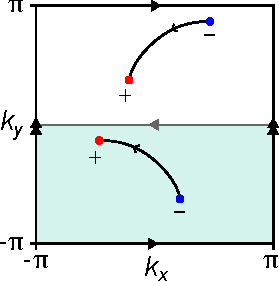
\includegraphics[width=.3\textwidth]{Images/BZ_basic}}
	\hfil
	\subcaptionbox{$-\pi/2 \leq k_y \leq \pi/2$}{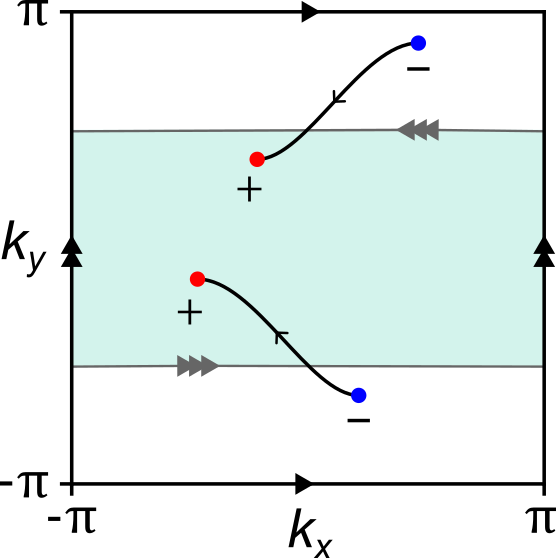
\includegraphics[width=.3\textwidth]{Images/BZ_mid}}
	\hfil
	\subcaptionbox{$-\pi \leq k_x \leq 0$}{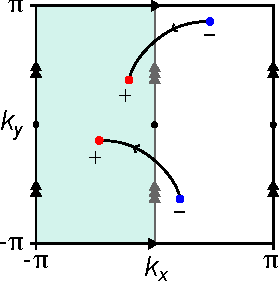
\includegraphics[width=.3\textwidth]{Images/BZ_left}}
	\caption{Top view of the 3D Brillouin torus (or 2D surface torus) for a given Weyl semimetal state obeying the glide symmetry in Equation~\eqref{eq:3D_glide}, with Weyl points and oriented Dirac strings (Fermi arcs) drawn in. Different parametrisations of the fundamental domain are shaded in teal: (a) the domain outlined in Ref.\ \cite{Fonseca-Vaidya_nonorientable}; (b) the same domain shifted in the $k_y$ direction; (c) a domain spanning the $k_y$ direction. Each of these domains is homeomorphic to $K^2\times S^1$ ($K^2$) under the boundary identifications shown. Note that the relative chirality of the two Weyl nodes in the fundamental domain changes under both alternative parametrisations.}
	\label{fig:BZ_param}
\end{figure}
For any given set of distinct Weyl points obeying the symmetry, it is possible in principle to achieve any relative chirality by reparametrising the fundamental domain. \red{This may mean that the charge of the Weyl points is fundamentally an $\N$ invariant on $K^2\times S^1$, but this is not clearly reflected in the cohomology description.} It should be noted that there do exist two planes that are of special significance, namely the so-called \emph{glide planes} at $k_x = 0$ and $k_x = \pm\pi$; these planes are (taken as a whole) invariant under the symmetry, and as such they cannot be excluded completely from any given parametrisation.

A similar point of confusion arises in explaining how the usual relation between Nielsen--Ninomiya and the Poincaré--Hopf theorem for vector fields breaks down. On the regular Brillouin torus, the factor $\h(\k)$ in the Bloch Hamiltonian can be considered a continuous vector field tangent to the torus. The Poincaré--Hopf theorem then tells us that the zeroes of such vector fields must have topological indices (corresponding to Weyl point chiralities) adding up to zero.

In the supplement to Ref.\ \cite{Fonseca-Vaidya_nonorientable}, the failure of Poincaré--Hopf is attributed to a discontinuity of the vector field at the planes $k_y=\pm\pi$ and $k_y=0$, see Figure~\ref{fig:Klein-discontinuity}.
\begin{figure}[htb!]
	\centering
	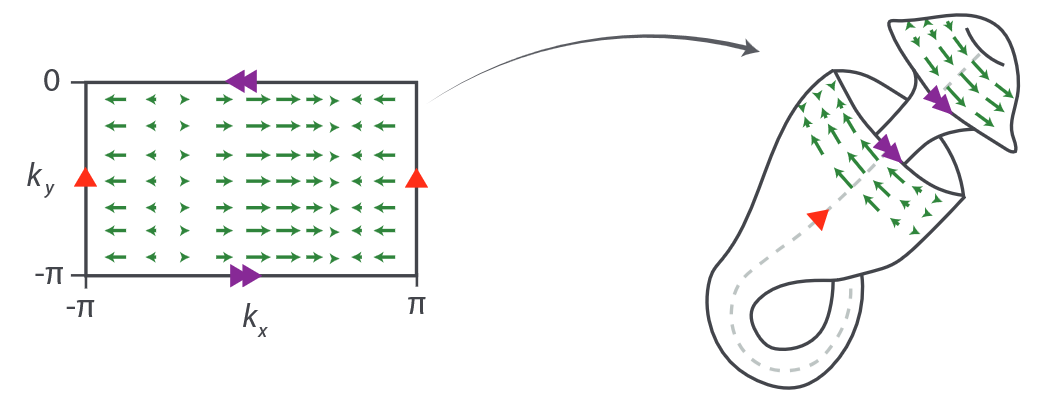
\includegraphics[width=.8\linewidth]{Images/Klein-discontinuity}
	\caption{Figure~from the supplement to Ref.\ \cite{Fonseca-Vaidya_nonorientable}. The $k_x$ component of an example $\h(\k)$ is mapped onto a $K^2$ slice of the fundamental Brillouin zone and then ``bent into shape'' to demonstrate discontinuity.
	}
	\label{fig:Klein-discontinuity}
\end{figure}
However, this mischaracterises the situation somewhat; in reality, $\h(\k)$ cannot be considered a well defined tangent vector field to $K^2\times S^1$ to begin with. This is illustrated in Figure~\ref{fig:BZ_vectors}: two vectors which point away from each other in the fundamental domain may instead point towards each other after applying the glide symmetry.
\begin{figure}[htb!]
	\centering
	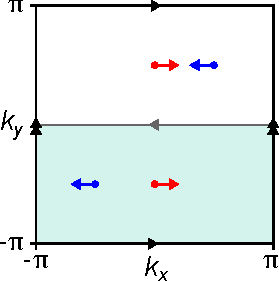
\includegraphics[width=.3\linewidth]{Images/BZ_vectors}
	\caption{Example vectors $\h(\k)$ on the glide symmetric Brillouin zone. Similar colours indicate that the vectors are related by glide symmetry.}
	\label{fig:BZ_vectors}
\end{figure}
As such, $\h$ should be thought of as a more abstract map $K^2\times S^1\to\R^3$ rather than a tangent vector field, and Poincaré--Hopf does not apply to such maps.\footnote{
	To be precise, $\h$ is a section of the trivial $\R^3$-bundle over $K^2\times S^1$, not of its tangent bundle. In the usual case of the torus, these descriptions are equivalent: $\T^3$ is parallelisable, i.e.\ $T\T^3\cong \T^3\times\R^3$. This is what allows Poincaré--Hopf to apply.}
{\color{red}
\st{In theory, one could construct a Hamiltonian starting from a proper tangent vector field to $K^2\times S^1$; this requires using gamma matrices that ``twist along'' with the tangent bundle of the manifold instead of the regular vector of Pauli matrices.}\footnote{\color{red}
	The proper construction is that of a Clifford algebra bundle over the tangent bundle, see Section 4.2 of Ref.\ \cite{Mathai_math-review}.}
[This may rely on the existence of a spin$^c$ structure, which probably does not exist in this case. This might also have implications for how ``physical'' a non-orientable BZ really is.]
}

A final point that merits clarification is the inclusion of a second glide symmetry. The supplement to Ref.\ \cite{Fonseca-Vaidya_nonorientable} discusses imposing Equation~\eqref{eq:3D_glide} together with a similar symmetry along the glide plane $k_y = 0$:
\begin{equation}
	H(k_x, k_y, k_z) = H(k_x + \pi, -k_y, k_z).
\end{equation}
It is claimed that this double symmetry subdivides the 3-torus into four copies of a different non-orientable manifold: namely $\RP^2\times S^1$, where $\RP^2$ is the real projective plane. This is broadly true, but it overlooks a seemingly innocuous detail: while the two glide symmetries have a free $\Z_2$ action on the torus individually, the action of the combined $\Z_2\oplus\Z_2$ symmetry group is no longer free. To be precise, there are four lines of high-symmetry points in the torus that are fixed by the diagonal subgroup of $\Z_2\oplus\Z_2$, similar to the time reversal invariant momenta discussed in Section \ref{sec:T-WSMs}; see Figure~\ref{fig:RP2-corners}.
\begin{figure}[htb!]
	\centering
	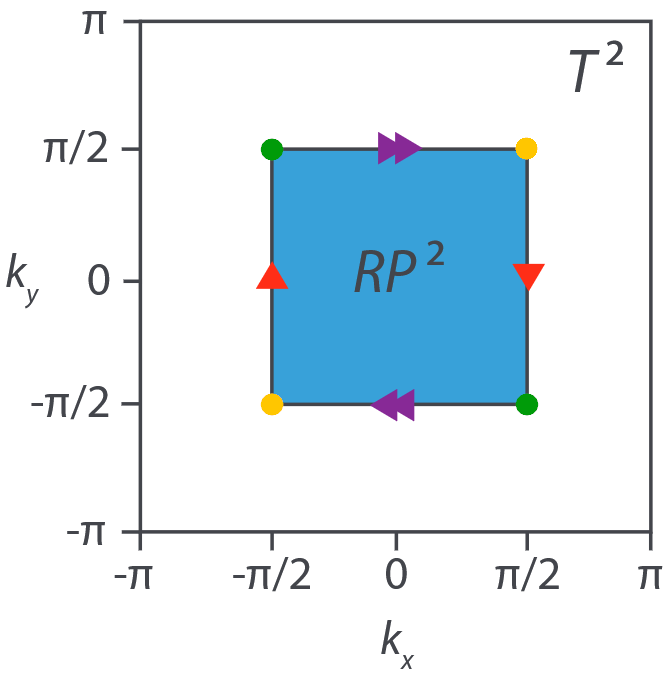
\includegraphics[width=.5\linewidth]{Images/RP2-corners}
	\caption{Figure~adapted from the supplement to Ref.\ \cite{Fonseca-Vaidya_nonorientable}. High-symmetry points (orange, green) exist for $k_x,k_y\in\{-\pi/2,\pi/2\}$; these points are fixed under simultaneous application of both glide symmetries. Similarly coloured points are related by a single glide symmetry and so they are identified on $\RP^2$.}
	\label{fig:RP2-corners}
\end{figure}
As a result, a Weyl point existing on one of these lines must have an even chirality, and it only has one symmetric partner in the 3-torus rather than the three one would expect from four identical copies of $\RP^2\times S^1$.\footnote{
	One can also argue that this must be the case topologically: if a manifold $M$ has an $n$-sheeted cover $\tilde{M}$, then the Euler characteristics of both spaces must be related by $\chi(\tilde{M}) = n\chi(M)$. Going to two dimensions, we find $\chi(\T^2) = 0$ and $\chi(\RP^2) = 1$, so that the former cannot cover the latter. Instead, the only possible covering space for $\RP^2$ is the double cover $S^2\to\RP^2$, since $\chi(S^2) = 2$.}
Such Weyl points are physically fine-tuned and are expected to split into pairs under perturbations. Nevertheless, additional symmetries may exist which force Weyl points to exist on these lines, in which case the exceptional behaviour becomes fundamental to the description. %TODO citation/remove?
Moreover, the notion of a fundamental Brillouin zone is predicated on a free group action in the main text of Ref. \cite{Fonseca-Vaidya_nonorientable}. As such, analysis of a purely $\RP^2\times S^1$ Brillouin zone cannot a priori be expected to provide the correct classification for this double glide symmetry. Indeed, similar to the case of time reversal in Section \ref{sec:T-WSMs}, a proper classification scheme should involve equivariant cohomology on the torus, bearing in mind the topological role of the high-symmetry points.\footnote{
	The mathematical description may be further complicated by the fact that the high-symmetry points are fixed only by a proper subgroup of the symmetry group. Beyond equivariant cohomology, it may be necessary to treat $\RP^2\times S^1$ as an \emph{orbifold} rather than a manifold, i.e.\ a space that encodes data about orbits of a group action. For example, the Euler characteristic of $\RP^2$ is zero as an orbifold. These spaces can be analysed using the highly specialised tool of \emph{orbifold cohomology}. \red{[On closer inspection, I'm not sure this is strictly true---most versions of orbifold cohomology seem to be an equivalent to (but perhaps more natural in this setting than) some equivariant cohomology.]}} %TODO citation
This analysis is somewhat beyond the scope of the present text, and in what follows we will restrict our attention to the case of a single glide symmetry.

\subsection{Classification scheme}

There are two main conceptual challenges that present themselves in attempting to apply consistent cohomology and homology frameworks to non-orientable systems, and in particular in developing a physical intuition for them. First of all, the analogy between second cohomology classes and Berry curvature $\Fc$ breaks down in this case, and a statement like Equation~\eqref{eq:2nd-cohom-t3} can no longer be taken to hold directly. %TODO clarify?
This is because differential forms like $\Fc$ cannot be integrated over non-orientable manifolds, and the associated (de Rham) cohomology group is actually real-valued---it cannot readily encode the $\Z_2$ invariants induced by changes in orientation. As an example, suppose we are trying to find an invariant for the 2D Klein bottle insulator obeying Equation~\eqref{eq:2D_glide}. Integrating a Berry curvature on $K^2$ directly is not well defined, while integrating over the entire Brillouin torus always yields zero: the integration is over two oppositely oriented areas. The correct $\Z_2$ invariant can be interpreted as integration with different signs on both halves of the torus, bearing in mind that the result is only gauge invariant mod 2. In order to capture this behaviour generally, we need to move to the richer but more abstract integer-valued cohomology. %TODO refer to appendix?

The second obstacle is that Poincaré duality is altered in this context. In Section \ref{sec:semimetal-topology} this form of duality was used to identify the familiar cohomology invariants with homology invariants, in the form of non-trivial oriented loops and Dirac strings. In a non-orientable system, this identification cannot be made directly; in this case, either the homology or the cohomology must be \emph{twisted} by the introduction of a \emph{local coefficient system} $\ext{\Z}$ \cites{Whitehead_Homotopy}{Hatcher_algebraic-topology}. Such a coefficient system compensates for the twist in orientation by tracking sign changes across the manifold. Introducing local coefficients on an $n$-manifold $M$ gives rise to the twisted homology and cohomology groups $H_k(M;\ext{\Z})$ and $H^k(M;\ext{\Z})$. Poincaré duality then takes the following forms \parencite[Thm. 3H.6]{Hatcher_algebraic-topology}:
\begin{align*}
	H_k(M;\ext{\Z}) &\cong H^{n-k}(M), \\
	H^k(M;\ext{\Z}) &\cong H_{n-k}(M).
\end{align*}
That is, twisting either one of the homology or cohomology restores Poincaré duality; if the homology is twisted, ordinary cohomology must be used and vice versa. When $M$ is orientable, the local coefficients become trivial and the original form of Poincaré duality is recovered from both relations.

Given the fact that Poincaré duality can be restored by twisting either the homology or the cohomology group, the correct classification of a non-orientable physical system hinges on making the correct choice between the two. Fortunately, there is a straightforward way to decide between the two in the case of a Weyl semimetal with an orientation-reversing $\Z_2$ symmetry. In this case, Poincaré duality is necessary in order to relate the chirality of Weyl points (which are cohomology invariants) to the orientation of their corresponding Dirac strings (which are the dual homology invariants). Under the orientation-reversing symmetry, Poincaré duality breaking manifests itself in the fact that the Weyl point chiralities are naturally reversed, while the orientation of Dirac strings is unchanged. This is illustrated schematically in Figure~\ref{fig:local_coefficients}.
\begin{figure}[htb!]
	\centering
	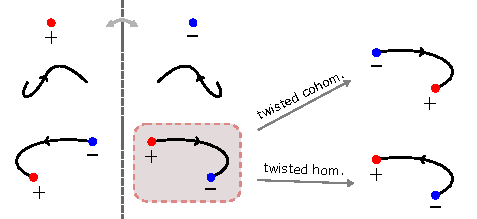
\includegraphics[width=.9\linewidth]{Images/local_coefficients}
	\caption{On the left, the action of an orientation-reversing symmetry (represented by the dashed mirror axis) is shown on a Weyl point [whose chirality is an invariant in $H^2(M\setminus W)$] and a Dirac string  [representing an invariant in $H_1(M,W)$]. The Weyl point has its chirality reversed, since the Chern number is a pseudoscalar; on the other hand, the Dirac string is mirrored but maintains its internal orientation. As a result, if the symmetry acts on a set of two Weyl points connected by a Dirac string, the resulting structure has a Dirac string whose orientation is inconsistent with the chirality of the Weyl points (shown in the shaded area)---this is a result of Poincaré duality breaking. This problem can be resolved in one of two ways: either the cohomology is twisted into $H^2(M\setminus W;\ext{\Z})$ to undo the chirality reversal, or the homology is twisted into $H_1(M,W;\ext{\Z})$ to reverse the Dirac string's orientation. Poincaré duality is restored in both cases; the correct approach depends on the physical setup.}
	\label{fig:local_coefficients}
\end{figure}
The decision of which group must be twisted can thus be made by noting how the chirality of Weyl points (outside of high-symmetry points) relates to that of their symmetric partners in the full Brillouin torus. To be precise, the presence of same-chirality pairs indicates that the (cohomological) Chern number is not reversed as expected, and the cohomology must be twisted. Meanwhile, pairs with opposite chiralities indicate that the cohomology behaves naturally, and the homology (i.e.\ the Dirac string orientations) must be twisted to follow suit.

As an example, we may apply this line of reasoning to the time reversal invariant Weyl semimetal from Section \ref{sec:T-WSMs}. This system is not usually thought of in terms of non-orientability, but the time reversal symmetry acts in an orientation-reversing way: an odd number (i.e.\ all three) of momentum directions is inverted, leading to a change of parity. Figure~\ref{subfig:TRS_orientation} illustrates that the effective Brillouin zone is indeed non-orientable.
\begin{figure}[htb!]
	\centering
	\subcaptionbox{\label{subfig:TRS_orientation}}{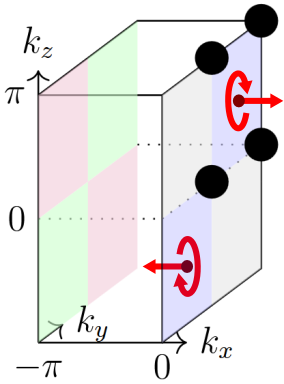
\includegraphics[width=.4\textwidth]{Images/TRS_EBZ_orientation}}
	\hfil
	\subcaptionbox{\label{subfig:TRS_Kramers}}{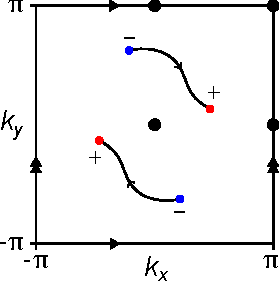
\includegraphics[width=.5\textwidth]{Images/Kramers_pairs}}
	\caption{(a) Figure~adapted from Ref.\ \cite{Thiang_equivariant}. The effective Brillouin zone under time reversal symmetry is half of $\T^3$, with additional identifications of the coloured areas as $k\sim -k$. The resulting space is non-orientable: a ``test particle'' with a given helicity is shown travelling out through the boundary at $\k = (0,\pi/2,\pi/2)\tran$, and reappearing at $\k = (0,-\pi/2,-\pi/2)\tran$ with the opposite helicity. (b) Top view of a time reversal invariant Weyl semimetal, featuring same-chirality Kramers pairs at conjugate momenta, indicating a twist in the cohomology. On the other hand, the orientation of Dirac strings is maintained by the symmetry, indicating ordinary (``untwisted'') homology.}
	\label{fig:TRS_twist}
\end{figure}
As discussed before, such systems feature Kramers pairs of Weyl points at opposite momenta related by $\k\leftrightarrow -\k$, both of which always have the same chirality; see Figure~\ref{subfig:TRS_Kramers}.
Again, these same-chirality pairs are an indication that the Chern numbers of Weyl points do not transform as expected, and so the cohomology must be twisted. It follows that the homology should not be twisted; this can also be seen directly from the fact that the Dirac strings in Figure~\ref{subfig:TRS_Kramers} have the same relative orientation. This description in terms of twisted cohomology and ordinary homology agrees exactly with the one given in Section \ref{sec:T-WSMs}, which was derived from more abstract vector bundle classification arguments in Ref.\ \cite{Thiang_equivariant}. In this particular case, direct calculation of the (co)homology groups on the effective Brillouin zone is complicated by the existence of high-symmetry points (i.e.\ the action of the symmetry is not free), which is why the authors of Ref.\ \cite{Thiang_equivariant} elect to use equivariant (co)homology on the full torus.

Returning to the case of a momentum-space glide symmetry, we can see from Figure~\ref{subfig:BZ_basic} that the situation is different here. Every Weyl point in the fundamental domain is related by symmetry to an oppositely charged point in the other half of the torus, while the orientation of Dirac strings is reversed under the symmetry. It follows that the classification of topological phases should rely on twisted \emph{homology}, and equivalently, ordinary cohomology. Since there is a proper fundamental domain in this case, there is no need to compute equivariant (co)homology groups, and we may instead rely on ordinary cohomology and twisted homology on $K^2\times S^1$.\footnote{\label{ft:eq_cohom}
	Formally speaking, equivariant cohomology of a space $M$ with a free action of the group $G$ is equivalent to ordinary cohomology on the quotient space $M/G$ \parencite[Cor. 9.6]{Tu_equivariant}.}

The choice of ordinary cohomology can be corroborated in two important ways. Firstly, the use of ordinary second cohomology classes indicates that we are classifying complex line bundles over the fundamental domain. An important insight from K-theory tells us that this is equivalent to classifying equivariant line bundles over the full torus \parencite[Prop. 2.1]{Segal_K-theory}.\footnote{
	This is related to footnote \ref{ft:eq_cohom} in the sense that K-theory is a \emph{generalised cohomology} theory.}
That is, we are classifying states that respect the symmetry directly. Secondly, the $\Z_2$ invariant found in Ref.\ \cite{Fonseca-Vaidya_nonorientable} on $K^2$-like slices of constant $k_z$ is recovered using ordinary cohomology, related to the fact that $H^2(K^2)\cong\Z_2$. Twisted cohomology would give a $H^2(K^2;\ext{\Z})\cong\Z$ invariant on these slices.

All in all, we find that the correct classification of semimetal phases in this system is given by the following Mayer--Vietoris sequence of cohomology groups on $M := K^2\times S^1$:
\begin{equation}\label{eq:MV-nonorientable}
	0 \to H^2(M) \to H^2\big(M\setminus W\big) \to H^2\left(\bigcup_{i=1}^k S_{w_i}^2\right) \to H^3(M) \to 0,
\end{equation}
where $S_{w_i}^2$ is a 2-sphere surrounding the Weyl point $w_i\in W$ as before. Equivalently, the classification may be given in terms of the following dual \emph{twisted} homology sequence:
\begin{equation}\label{eq:homology-sequence-nonorientable}
	0 \to H_1(M;\ext{\Z}) \to H_1\big(M, W;\ext{\Z}\big) \overset{\partial}{\to} H_0(W;\ext{\Z}) \to H_0(M;\ext{\Z}) \to 0.
\end{equation}
In what follows, we will provide explicit computations of these groups and discuss the associated invariants.


\subsection{Computing invariants}

The use of ordinary cohomology groups in the Mayer--Vietoris sequence \eqref{eq:MV-nonorientable} means calculations are relatively straightforward, and standard techniques such as cellular cohomology can be applied. \red{[Should I make a small Appendix B containing an example cellular cohomology calculation?]} Using these methods, we calculate the sequence to be
\begin{equation*}
	0\to \mathbb{Z}\oplus\mathbb{Z}_2 \to \mathbb{Z}^{1+k}\oplus\mathbb{Z}_2 \to \mathbb{Z}^k \to \mathbb{Z}_2 \to 0.
\end{equation*}

%TODO

{\color{blue}
\begin{itemize}	
	\item Cohomology is easy to compute, but its dual twisted homology offers a very intuitive perspective of the invariants, demonstrating how the $\Z^3$ invariant on a 3D Chern insulator gets reduced to a $\Z\oplus\Z_2$ under this symmetry. The $\Z_2$ factor is precisely the $\Z_2$ invariant discussed by Fonseca, Vaidya et al. This intuition is especially clear when viewed as twisted equivariant homology on $\T^3$. [Include pictures of the action of the symmetry on the three basic homology invariants on $\T^3$.]
	
	\item Under this description, the semimetal Mayer--Vietoris sequence becomes
	\begin{equation*}
		0\to H^2(K^2\times S^1) \to H^2(K^2\times S^1\setminus W) \to H^2(S_W) \to H^3(M) \to 0,
	\end{equation*}
	which can be calculated explicitly (using e.g. cellular (co)homology) as
	\begin{equation*}
		0\to \mathbb{Z}\oplus\mathbb{Z}_2 \to \mathbb{Z}^{1+k}\oplus\mathbb{Z}_2 \to \mathbb{Z}^k \to \mathbb{Z}_2 \to 0.
	\end{equation*}
	From the $\Z_2$ in the last term, we immediately recover the $\Z_2$ charge cancellation no-go theorem. It also becomes clear that a single Weyl point may carry non-trivial topology (i.e. already adds a factor to the group of invariants).
\end{itemize}

Additionally:

\begin{itemize}
	\item The description can easily be extended to a 2D type AIII Klein bottle WSM with chiral symmetry; in this case, 1st cohomology invariants (winding numbers) are dual to twisted 1st homology invariants (Fermi arcs/loops).
	
	\item More elementary systems such as 3D type A with inversion symmetry also exhibit non-orientable EBZs, but in this case the description is complicated by the existence of fixed points (the TRIM).
	
	\item Applicability of this description is probably limited under addition of non-trivial additional bands, e.g. 4-band models incorporating spin and orbital degrees of freedom. The full scope of applicability is somewhat of an open question at this point. (E.g., how well are 2D chiral WSMs described by this homology picture?)
\end{itemize}
}



{\color{red}
\section*{Notes}
Concepts explored in early personal notes:
\begin{itemize}
	\item Calculations of (co)homology and semimetal MV sequence for manifolds in $\geq2$ dimensions:
	\begin{itemize}
		\item All compact surfaces without boundary, i.e.\ the surfaces $M_g$ and $N_g$
		
		\item All spaces of the form $M = K^2 \times \T^{d-2}$
	\end{itemize}
	
	\item The map $\Sigma:H^{d-1}(\bigsqcup_{k}S^{d-1})\to H^d(M)$ in the semimetal MV has a clear interpretation in terms of total charge in the (orientable) $d=3$ case. This would provide a clear picture of the total charge cancellation in the orientable case ($H^d(M) = \Z$ in general) vs. the mod 2 charge cancellation in the non-orientable case ($H^d(M) = \Z_2$ in general).
	
	\item However, $\Sigma$ and the other maps in the MV sequence are difficult to interpret in the $\chi\neq 0$ case (maybe even generally for odd dimensions). Taking the oriented case as an example, the MV sequence ends as
	\begin{align*}
		H^{d-1}(M\setminus\Delta)\ \rightarrow\ H^{d-1}\left(\bigsqcup_{k}S^{d-1}\right) \cong \Z^k\ \overset{\Sigma}{\rightarrow}\ H^d(M) \cong \Z
	\end{align*}
	so that the ``charge configuration'' in $\Z^k$ must map to 0 by $\Sigma$ in order to descend from the semimetal, regardless of whether $\chi=0$.
	
	\item This may imply that the Bloch vector field carries more topological information about the total charge than the MV sequence (which makes sense since it generates \emph{all} homology groups of the valence bundle, and all Betti numbers factor into $\chi$). As a concrete example, consider $M=S^2$ with a single puncture of charge $+2$. The punctured sphere is topologically a disc, so that the valence bundle must be trivial, while the Bloch vector field is topologically non-trivial in the sense that it has an index $+2$ singularity. In addition, all relevant $H_n(A)\oplus H_n(B)$ are zero, so that the semimetal MV reduces to the statement that $H_2(S^2)\cong H_1(S^1)$.
	
	\item It may even be the case that the valence bundle cannot be generated from the Bloch vector field in the $d=2$ case; it's probably worth studying the $d\in\set{3,4,5}$ cases (pullback of some universal bundle) to learn more about this. The $d=3$ case should be especially helpful in understanding how the valence bundle arises from the vector field.
	
	\item A complicating factor in the non-orientable case is that the homology groups are different from the cohomology groups, since the torsion moves up one dimension. This makes the homological semimetal MV different from the cohomological one (it's a short exact sequence in $d\geq3$!), and this leads to additional challenges in interpretation.
	
	\item The map $H: \R^3\to\la[su](2),\ \vec{h}\mapsto \vec{h}\cdot\vec{\sigma}$ is an isomorphism of Lie algebras, with the cross product as a Lie bracket on $\R^3$. Still the vector field is discontinuous on a non-orientable manifold, while $H$ is not. This suggests an alternative approach for constructing the valence bundle: consider $h$ as a map $M\to\R^d$ instead of an element of $\vct(M)$, and then pull back the universal bundle along the unit map $\hat{h}:M\setminus\Delta\to S^{d-1}$. That is, we detach $\vec{h}$ from the tangent bundle and consider it a more abstract map. An added ``benefit'' of this is that we lose all coordinate dependence. However, this may also be a downside in the sense that the map will not be subject to the same constraints (Poincaré--Hopf etc.) that the vector field is; for example, $S^2\to\R^2,\ x\mapsto(1,0)$ is a perfectly valid map that would violate the hairy ball theorem as a vector field (and this is a result of being unable to cover $S^2$ by a single chart). At this point the question may become more about which description is more physical in nature, and the non-orientable Weyl point paper\cite{Fonseca-Vaidya_nonorientable} seems to imply there may be more to the $h:M\to\R^3$ story. It also seems to agree better with the intuition of an applied external potential removing all Weyl nodes -- something that's impossible for $\chi\neq0$ if charge corresponds to vector field index. It also explains how the valence bundle can be trivial on the once punctured $S^2$.
	
	\item In light of the previous point, this may be an important observation: every $d$-manifold $M$ with $\chi(M)=0$ admits a nowhere-vanishing vector field (\href{https://math.stackexchange.com/questions/47370/if-a-manifold-m-has-zero-euler-characteristic-there-is-a-non-vanishing-vector-f}{link}). \st{This may imply that the vector field description is equivalent to the map to $\R^d$ in these cases, though one needs to be careful about charts. It would be good to find or write a (dis)proof for something like $\vct(M)\cong\Cinf(M,\R^d)$ (or similar for non-vanishing maps) in this case. Or more specifically:}
	\[
		\st{\big[M\setminus\Delta,S^{d-1}\big] \stackrel{?}{\cong} \Set{\vec{h}\in\vct(M\setminus\Delta) | \text{$\vec{h}$ is non-vanishing}}}
	\]
	Update: I think the real requirement for equivalence is that the base manifold $M$ is parallelisable (i.e.\ has a trivial tangent bundle), since we're essentially using a trivial $\R^d$-bundle in this construction.
	
	\item Any smooth $d$-manifold can be given a CW complex structure with one $d$-cell (\href{https://mathoverflow.net/questions/120799/manifolds-admitting-cw-structure-with-single-n-cell}{link}). On this $d$-cell there is an exact correspondence between vector fields and maps to $\R^d$, since it can be embedded in $\R^d$. What distinguishes the two is how points on the boundary of the $d$-cell are identified with each other; this determines whether the ``vectors'' need to change orientation. To illustrate:
	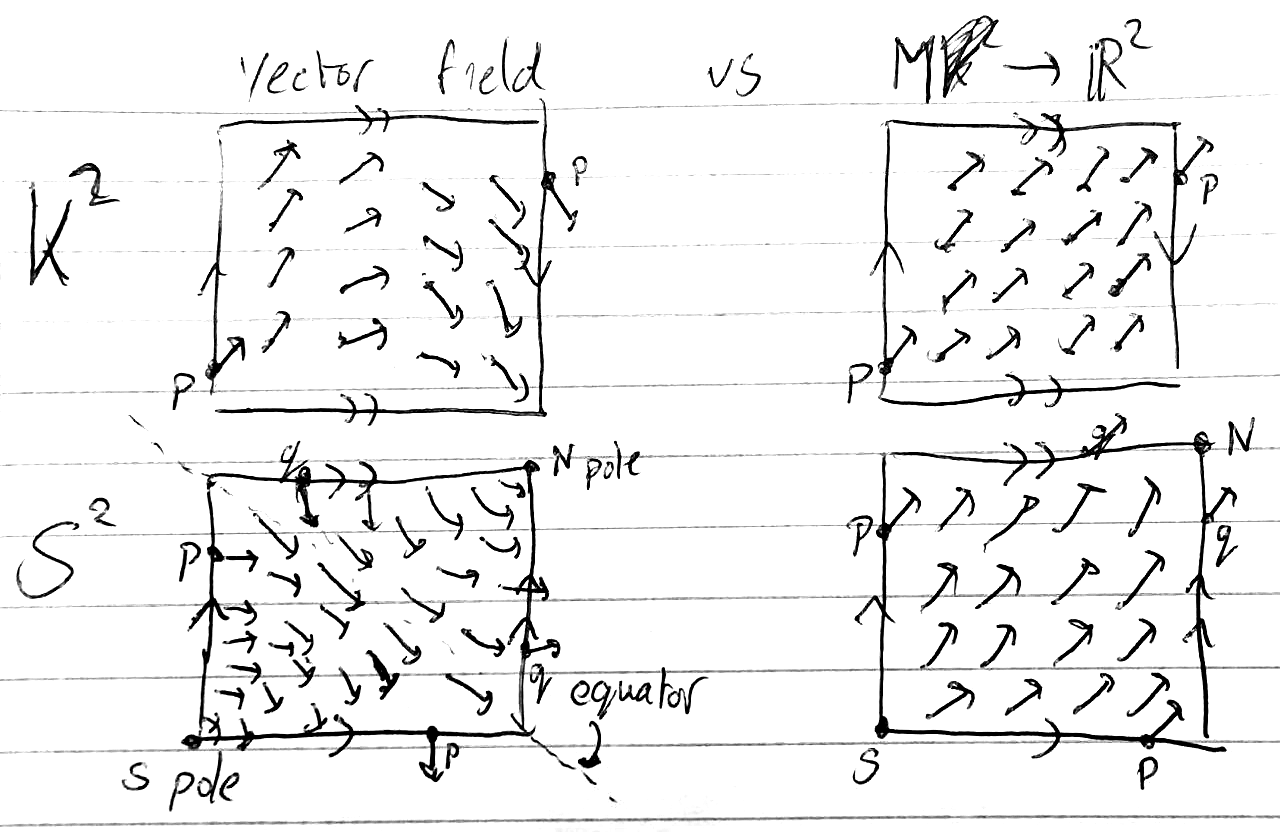
\includegraphics[width=.9\textwidth]{Images/vectorfield-vs-map}
	
	\item On any orientable manifold, the Stokes' theorem argument shows that the total charge must be zero regardless of Euler characteristic:
	\[
		\sum_{\alpha}w(S_\alpha) = \sum_{\alpha}\int_{S_\alpha} c_1(E) = \sum_{\alpha}\int_{S_\alpha}\frac{\Tr\Fc}{2\pi} = \int_{B'} \dd{\frac{\Tr\Fc}{2\pi}} = 0
	\]
	where the last equality holds by the Bianchi identity for the trace. This means the valence bundle cannot be a pullback along a tangent vector field for $\chi\neq0$.
	
	On a non-orientable manifold, this argument doesn't hold since the integral over $B'$ isn't well defined.
	
	\item Total chirality isn't well defined on a non-orientable manifold (at least in odd dimensions, not sure how to interpret even dimensions). Still there is charge cancellation in the form of Fermi arcs etc.; it may take moving to a different homology system to get the full picture, such as homology with local coefficients or equivariant homology. (See e.g. \cite{Thiang_equivariant})
	
	\item It may be worth classifying which manifolds are candidates for physical material Brillouin zones; I have a feeling that this might be restricted to those manifolds for which the $n$-torus is a covering space. In this case a full classification of symmetries on the torus (and e.g. their related equivariant homologies) would be sufficient to classify all material topologies. This classification is related to space group symmetries.
\end{itemize}
}  % end red colour